%http://cs.pugetsound.edu/~jross/courses/cs240/project/requirements/
%Animation Group
\documentclass[12pt]{article}
\usepackage{graphicx}
\begin{document}




% Front Page
\begin{titlepage}
	\begin{center}
	\huge  Edith \\
	\vspace*{\fill}%
 	\huge \textsc{\textbf{Animation Team \\Requirement Specifications} }	
	\bigskip 
	\rule{130mm}{.1pt}
	\textsc{\textbf{September 25 2013 \\ Revised: September 25 2013} \\ }	
	\vspace*{\fill}%
	Eric Lund \\
	Kramer Canfield \\ 
	Zeke Rosenberg \\
	Calder Whiteley \\
	Jon Youmans
	\end{center}
	\end{titlepage}

% Next page

%Executive Summary
\section{\emph{Executive Summary}}
Our Summary will be placed here!Our Summary will be placed here!Our Summary will be placed here!Our Summary will be placed here!Our Summary will be placed here!Our Summary will be placed here!Our Summary will be placed here!Our Summary will be placed here!Our Summary will be placed here!


%Introduction
\section{\emph{Introduction}}%Create a section for the introduction
	\subsection{Edith}
Details hereDetails hereDetails hereDetails hereDetails hereDetails hereDetails hereDetails hereDetails hereDetails hereDetails hereDetails hereDetails hereDetails hereDetails hereDetails hereDetails hereDetails hereDetails here
	\subsection{Module}
	Details hereDetails hereDetails hereDetails hereDetails hereDetails hereDetails hereDetails hereDetails hereDetails hereDetails hereDetails hereDetails hereDetails hereDetails hereDetails hereDetails hereDetails hereDetails hereDetails hereDetails hereDetails hereDetails hereDetails hereDetails hereDetails hereDetails hereDetails hereDetails hereDetails hereDetails hereDetails hereDetails hereDetails hereDetails hereDetails hereDetails hereDetails here
	\subsection{Purpose}
	Details hereDetails hereDetails hereDetails hereDetails hereDetails hereDetails hereDetails hereDetails hereDetails hereDetails hereDetails hereDetails hereDetails hereDetails hereDetails hereDetails hereDetails hereDetails here	Details hereDetails hereDetails hereDetails hereDetails hereDetails hereDetails hereDetails hereDetails hereDetails hereDetails hereDetails hereDetails hereDetails hereDetails hereDetails hereDetails hereDetails hereDetails here


% Use Cases
\section{\emph{Functional Requirements}}
	\subsection{"Use Case 1 NAME"}
\begin{enumerate}
  \item Actor
  \begin{enumerate}
  		\item Actor here
   		 \item Or here
  \end{enumerate}
  \item Preconditions/Assumptions
  \begin{enumerate}
   		 \item Preconditions 
   		 \item Assumptions
  \end{enumerate}
  \item Flow of Events
  \begin{enumerate}
   		 \item Flow here
   		 \item Sun Flows?
  \end{enumerate}
  \item Alternatives
  \begin{enumerate}
    		\item Flows that deviate from the main flow. "Exceptions"
    		\item More here
  \end{enumerate}
  \item  Postconditions
  \begin{enumerate}
    		\item Postconditions
    		\item More here
  \end{enumerate}
\end{enumerate}

	\subsection{"Use Case 2 NAME"}
\begin{enumerate}
  \item Actor
  \begin{enumerate}
  		\item Actor here
   		 \item Or here
  \end{enumerate}
  \item Preconditions/Assumptions
  \begin{enumerate}
   		 \item Preconditions 
   		 \item Assumptions
  \end{enumerate}
  \item Flow of Events
  \begin{enumerate}
   		 \item Flow here
   		 \item Sun Flows?
  \end{enumerate}
  \item Alternatives
  \begin{enumerate}
    		\item Flows that deviate from the main flow. "Exceptions"
    		\item More here
  \end{enumerate}
  \item  Postconditions
  \begin{enumerate}
    		\item Postconditions
    		\item More here
  \end{enumerate}
\end{enumerate}

\subsection{UML}
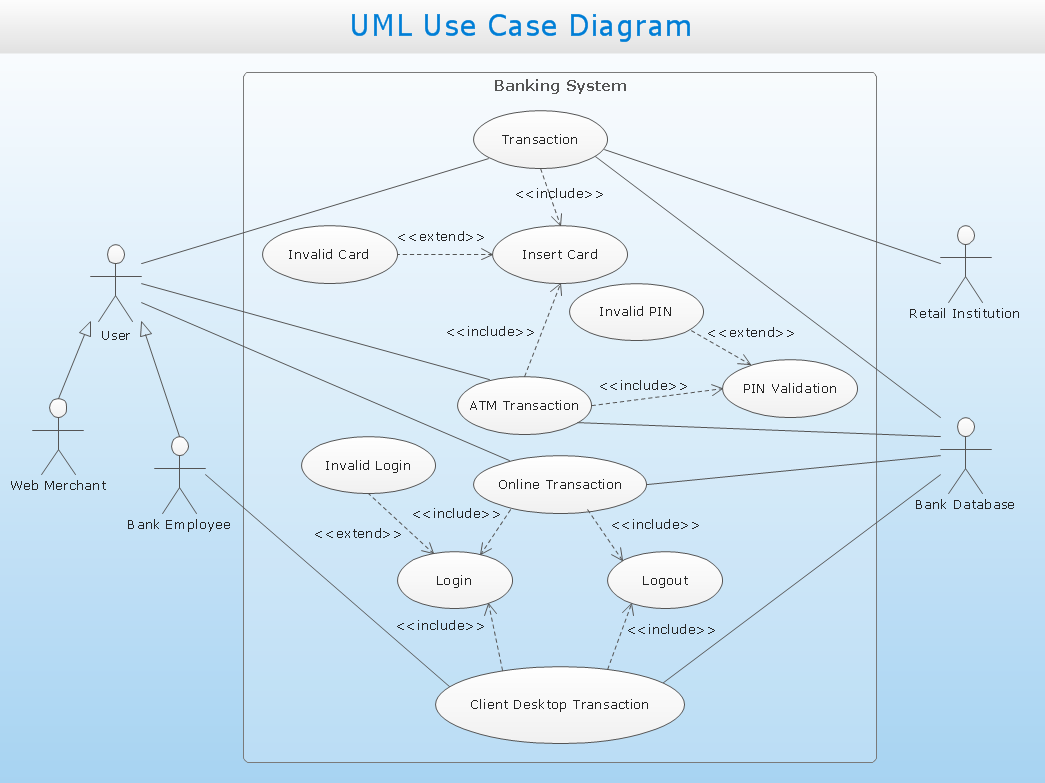
\includegraphics[scale=.5]{EXAMPLEUML.png}
Caption of UML? 



%Nonfunctional Requirements
\section{\emph{Nonfunctional Requirements}}
List and briefly describe (in a sentence or two) the nonfunctional requirements for your product. Try to describe the nonfunctional requirements in a testable manner; how will you know if you've made the system "easy to use"?

%Glossary/References
\section{\emph{Glossary/References}}
Finally, be sure to define the specialized terms you use (if any!), and to include citations to any references you make (e.g., if you reference any other systems as comparison points). Always provide proper attribution to other people's work.

\end{document}